\documentclass[times, utf8, diplomski]{fer}
\usepackage{booktabs}
\usepackage[croatian]{babel}
\usepackage[utf8]{inputenc}
\usepackage{pdfpages}

\setcounter{secnumdepth}{3}
\setcitestyle{numbers}
\graphicspath{ {./images/} }

\begin{document}

\thesisnumber{1373}

\title{Analiza i usporedba sigurnosnih mehanizama u Internetu stvari}

\author{Filip Ptiček}

\maketitle

% Ispis stranice s napomenom o umetanju izvornika rada. Uklonite naredbu \izvornik ako želite izbaciti tu stranicu.
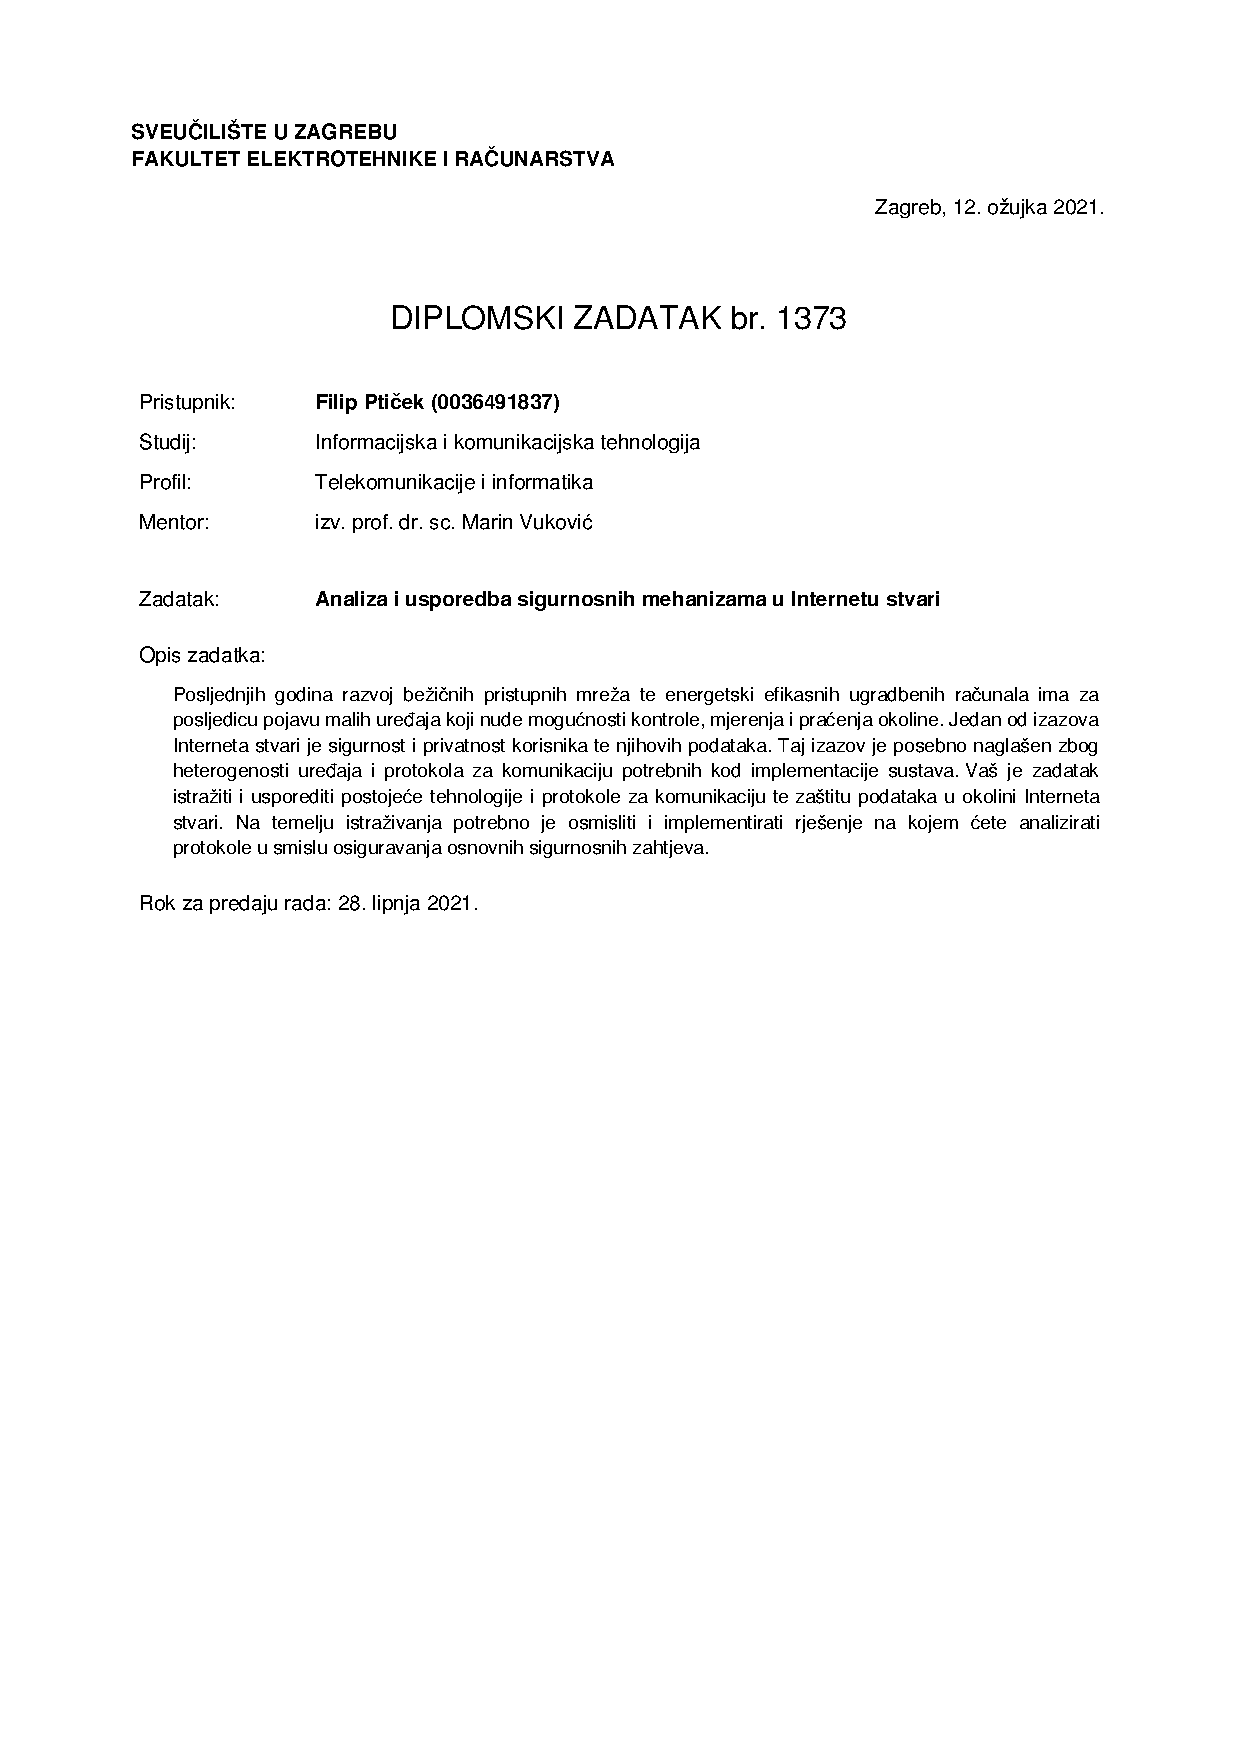
\includepdf[pages=-,fitpaper=true]{zadatak.pdf}

% Dodavanje zahvale ili prazne stranice. Ako ne želite dodati zahvalu, naredbu ostavite radi prazne stranice.
\zahvala{}

\tableofcontents

\chapter{Uvod}
Uvod u rad

\chapter{Internet stvari}

\section{Definicija}
a

\section{Model IoT sustava}
a

\section{Čimbenici u sustavu}
a

\section{Programske platforme}
a

\section{Otvorena pitanja}
a

\subsection{Sigurnost}
a

\subsection{Privatnost}
a

\subsection{Skalabilnost}
a

\subsection{Decentraliziranost}
a

\section{Primjene}
a

\subsection{Područja primjene}
a

\subsection{Zahtijevi sustava s obzirom na primjenu}
a

\section{Trendovi}
a


\chapter{Sigurnosni zahtijevi u Internet stvarima}

\section{OWASP Top 10}
The Open Web Application Security Project® (OWASP) je neprofitna organizacija čiji je cilj napredak i poboljšanje računalne sigurnosti informacijskih sustava. OWASP kroz svoje projekte otvorenog koda vođenih putem razvojne zajednice radi na poboljšanju sigurnosti Interneta.

\emph{OWASP Internet of Things Project} je projekt osmišljen kako bi pomogao proizvođačima, programerima i potrošačima bolji uvid i razumijevanje u sigurnosne probleme vezane uz Internet stvari. Na taj način korisnici u bilo kojem dijelu razvojnog procesa mogu donositi bolje odluke kod razvoja, deployanja i pristupanja tehnologijama Interneta stvari.\citep{owasp1} 2018. godine izlazi \emph{OWASP IoT Top 10} lista koja reprezentira deset najčešćih ranjivosti Internet stvari sustava. Svih deset sigurnosnih ranjivosti su navedeni u nastavku uz opis sigurnosnih zahtijeva koji bi trebali spriječiti te ranjivosti i sigurnosne propuste. 

\subsection{Slabe, pogodljive ili tvrdo kodirane lozinke}
Prvi navedeni sigurnosni problemi kod Internet stvari sustava su vezni uz lozinke. Kako bi se uređaju moglo pristupiti i naknadno ga konfigurirati, uređaji dolaze s korisničkim računima koji služe korisnicima kako bi ih mogli upariti sa željenim sustavim ili kako bi proizvođač mogao upravljati uređajem u slučaju pomoći korisnicima ili ažuriranja uređaja. Za pristup tom korisničkom računu uređaja je potrebna lozinka koju krajnji korisnik kod prve upotrebe treba postaviti. Navike korisnika su većinom da iskoriste njima dobro poznatu lozinku koju koriste i za svoje druge korisničke račune. Ako napadač dobije pristup jednoj njihovoj lozinci ima i pristup ostalim računima. Na taj način se pristup korištenim uređajima koji imaju isto korisničko ime ili e-mail adresu i lozinku uvelike olakšava. Korisnici imaju i naviku koristiti slabe lozinke koje su vrlo česte i jako lako pamtljive. Tako su neke od najčešće korištenih lozinka jednostavni nizovi numeričkih znakova ili nizovi znakova na tipkovnici poput: 123456, 123456789, qwerty, ili sam engleski prijevod lozinke \engl{password}.\citep{pass1}. Napadi na lozinke se provode putem takozvanih \emph{brute force} napada. Kako je procesna snaga današnjih računala dosegla vrlo visoke brzine računanja, tako se jednostavne i kratke lozinke mogu pogoditi u vrlo kratkom vremenu.

Ovakvi propusti ne zaobilaze ni proizvođače samih sustava i uređaja. Kod proizvodnje proizvođači na uređaje postavljaju iste lozinke za sve uređaje kako bi kod testiranja ispravnosti lakše pristupili istima. Jedan od najboljih pokazatelja takvog pristupa su usmjerivači/modemi telekom operatera za pristup Internetu koji imaju postavljenu istu zadanu lozinku i korisničko ime poput "admin" ili "user" koju krajnji korisnici uređaja nikada ne promjene. Problem se također pojavljuje i u tvrdo kodiranim \engl{hard coded} lozinkama. Proizvođači postave takve lozinke na uređaje kako bi se uređaji mogli nesmetano povezati s vanjskim servisima, kako bi se proizvođači povezli na uređaj zbog otklanjanja pogrešaka ili kao način za vanjsko upravljanje uređaja. Ako napadač ima fizički pristup uređaju on može skenirati memoriju i pomoću raznih alata pronači lozinku spremljenu na samom uređaju. A kako prozivođači najvjerojatnije koriste istu lozinku za sve iste modele uređaja, napadač ima lak način za pristup i ostalim istim uređajima.

Kako bi se spriječila ova vrsta ranjivosti neki od sigurnosnih zahtijeva koji bi se trebali pratiti su sljedeći. Korisnici bi kod prve upotrebe uređaja trebali promjeniti zadanu lozinku koristeći duge, kompleksne i jedinstvene nizove znakova. Najjednostavniji način postići te zahtijeve je korištenjem upravitelja lozinkama. Oni daju mogućnost generiranja lozinki uz mogućnost spremanja istih bez potrebe da korisnik mora pamtiti sve jedinstvene i duge lozinke. Što se tiče zahtijeva sa strane prozivođača, oni bi trebali razriješiti bolje načine upravljanja uređajima kako bi se izbjeglo korištenje istih ili čak tvrdo kodiranih lozinka za pristup uređaju ili vanjskim servisima. Također bi proizvođači trebali upozoriti korisnika kod uspostave uređaja da promijeni zadanu lozinku.

\subsection{Nesigurne mrežne usluge}
Internet stvari uređaji koriste razne mrežne usluge kako bi mogli komunicirati s vanjskim servisima. Kako je moguće pristupiti tim uređajima putem Interneta potrebno je pravilno osigurati sigurnost tih mrežnih usluga koje se izvršavaju. Neautoriziran pristup preko usluga iskorištavajući zadane lozinke, otvorene mrežne priključke te nepravilno podešeni vatrozidi dozvoljavaju napadaču da dobije pristup uređajima i poslužiteljima. Takvi napadi dozvoljavaju izvršavanje malicioznog koda, iskorištavanje uređaja za botnet, krađu podataka ili onesposobljavanje sustava.
%Expand a little bit

Neki od sigurnosnih mjera koje se mogu poduzeti za osiguravanje mrežnih usluga su: \begin{itemize}
    \item korištenje zasebne lokalne mreže za sve pametne uređaje,
    \item spajati uređaje na isključivo sigurne mreže,
    \item instaliranje regularnih softverskih ažuriranja,
    \item isključivanje svih usluga koje pružaju vanjski pristup uređaju,
    \item isključivanje nepotrebnih mrežnih priključaka i usluga,
    \item isključivo korištenje protokola koji koriste enkripciju.
\end{itemize}

\subsection{Nesigurna sučelja ekosustava}
Nesigurna web sučelja, pozadinski API-jevi, servisi u oblaku i mobilna sučelja, koja dozvoljavaju komunikaciju i interakciju s uređajem, čine sveukupni ekosustav Internet stvari. Kompromitacija bilo kojeg dijela sustava može uzrokovati i kompromitaciju cijelokupnog sustava. Ranjivost kod načina autorizacije i autentifikacije između uređaja i poslužitelja ili korisnika mobilnih i web aplikacija i poslužitelja su jedan od vektora napada na sustav. Također nedostatak ili korištenje slabe enkripcije kod komunikacije može uzrokovati da napadač presretne i iskoristi sakupljene informacije za napad. Nedostatak pravilnog filtriranja ulazno/izlaznih podataka može dovesti do napada poput SQL injekcije. Još jedan projekt OWASP organizacije je \emph{OWASP Top 10 Web Application Security Risks} koji nudi popis najčešćih ranjivosti za web i mobilne aplikacije. Nesigurna sučelja ekosustava imaju direktnu poveznicu s tim ranjivostima koje su: \begin{itemize}
    \item injekcije (SQL, NoSQL, OS, LDAP),
    \item neispravna autentifikacija,
    \item izlaganje osjetljivih podataka,
    \item XML External Entities(XXE) napadi,
    \item neispravna autorizacijska kontrola,
    \item pogrešna konfiguracija servisa,
    \item Cross-Site Scripting(XSS),
    \item nesigurna deserijalizacija podataka,
    \item korištenje bibilioteka i komponenta s poznatim sigurnosnim ranjivostima,
    \item nedovoljno korištenje logova i praćenja sustava.\citep{owasp2}
\end{itemize}

Pravilno podešavanje autorizacije i autentifikacije korisnika, ali i uređaja je najvažniji način osiguravanja raznih sučelja ekosustava. Filtriranje ulaznih i izlaznih podataka spriječava napade injekcijom, pravilno podešavanje poslužitelja da koriste pravilne enkripcijske načine komunikacije dozvoljavaju privatnu i sigurnu komunikaciju. Kroz cijeli ekosustav je potrebno i uspostava logiranja i praćenja sustava kako bi se na vrijeme otkrili nepravilna ponašanja unutar samog sustava.

\subsection{Nedostatak mehanizama za sigurnosna ažuriranja}
a

\subsection{Upotreba nesigurnih ili zastarijelih komponenti}
a

\subsection{Nedovoljna zaštita privatnosti}
a

\subsection{Nesigurni prijenos i pohrana podataka}
a

\subsection{Nedostatak mogućnosti upravljanja uređajima}
a

\subsection{Nesigurne zadane postavke}
a

\subsection{Nedostatak fizičke sigurnosti}
a

\section{Primjeri sigurnosnih napada i propusta}
a

\chapter{Analiza i usporedba protokola}

\section{IoT stack}
Iot stack

\section{Senzori i uređaji}
Senzori

\subsection{Analiza uređaja}
Uređaji

\subsubsection{Senzori s komunikacijskim modulom}
a

\subsubsection{Pristupni uređaji}
a

\subsection{Usporedba sigurnosnih mehanizama i primjena}
a

\section{Sloj podatkovne poveznice}
a

\subsection{Analiza protokola}
a

\subsubsection{WiFi}
a

\subsubsection{BLE}
a

\subsubsection{RFID\textbackslash NFC}
a

\subsubsection{ZigBee}
a

\subsubsection{LTE}
a

\subsubsection{SigFox}
a

\subsubsection{LoRaWan}
a

\subsection{Usporedba sigurnosnih mehanizama i primjena}
a

\section{Mrežni sloj}
a

\subsection{Analiza protokola}
Neki protokoli

\subsubsection{IPv4}
a

\subsubsection{IPv6}
a

\subsection{Usporedba sigurnosnih mehanizama i primjena}
a

\section{Transportni sloj}
a

\subsection{Usporedba primjena protokola}
a

\section{Aplikacijski sloj}
a

\subsection{Analiza protokola}
a

\subsubsection{HTTP/S}
a

\subsubsection{COAP}
a

\subsubsection{MQTT}
a

\subsection{Usporedba sigurnosnih mehanizama i primjena}
a

\chapter{Sustav za praćenje tjelesne temperature}

\section{Arhitektura sustava}
a

\section{Korišteni razvojni alati i uređaji}
a

\section{Opis rada sustava}
a

\section{Sigurnostna analiza sustava}
a


\chapter{Zaključak}
Zaključak.

\bibliographystyle{fer}
\bibliography{literatura}

\begin{sazetak}
Sažetak na hrvatskom jeziku.

\kljucnerijeci{Ključne riječi, odvojene zarezima.}
\end{sazetak}

% TODO: Navedite naslov na engleskom jeziku.
\engtitle{Title}
\begin{abstract}
Abstract.

\keywords{Keywords.}
\end{abstract}

\end{document}